%% Author: Leighton Pritchard
%% Copyright: James Hutton Institute
%% 2015-03-07: Slides for teaching at University of Dundee, 17th March 2015
%% This presentation was an invited lecture on comparative genomics and visualisation
%% for the BS32010 course.

%% UNCOMMENT FOR SLIDES
\documentclass[table]{beamer}
\mode<presentation>

%% UNCOMMENT FOR HANDOUTS
%\documentclass[handout]{beamer}
\usepackage{handoutWithNotes}
\pgfpagesuselayout{4 on 1 with notes}[a4paper,border shrink=5mm]

%% GENERIC STYLE SETTINGS BELOW
\usetheme{default}
\usepackage{listings}
\usepackage{multirow}
\usepackage{xcolor}
\usepackage{hyperref}
%\usepackage[multiple]{footmisc}

\usebackgroundtemplate{

\includegraphics[width=\paperwidth,height=\paperheight]{images/hutton_background}
}
%% PRESENTATION CONFIGURATION PARAMETERS %%%%%%%%%%%%%%%%%%%%%%%%%%%%%%%%%%%%%%%
%\titlebackgroundfile{images/hutton_title}
%\framebackgroundfile{images/hutton_background}
\definecolor{hutton_green}{HTML}{78A22F}
\definecolor{hutton_purple}{HTML}{872175}
\definecolor{hutton_blue}{HTML}{569BBE}
\definecolor{olive}{rgb}{0.3, 0.4, .1}
\definecolor{fore}{RGB}{249,242,215}
\definecolor{back}{RGB}{51,51,51}
\definecolor{title}{RGB}{255,0,90}
\definecolor{dgreen}{rgb}{0.,0.6,0.}
\definecolor{gold}{rgb}{1.,0.84,0.}
\definecolor{JungleGreen}{cmyk}{0.99,0,0.52,0}
\definecolor{BlueGreen}{cmyk}{0.85,0,0.33,0}
\definecolor{RawSienna}{cmyk}{0,0.72,1,0.45}
\definecolor{Magenta}{cmyk}{0,1,0,0}
\usefonttheme{structurebold}
\setbeamercolor{alerted text}{fg=orange}
\setbeamercolor{background canvas}{bg=white}
\setbeamercolor{block title}{bg=hutton_purple}
\setbeamercolor{frametitle}{fg=hutton_purple}
\setbeamercolor{title}{fg=black}
\setbeamercolor{titlelike}{fg=hutton_green}
\setbeamercolor{author}{fg=hutton_purple}
\setbeamercolor{author in head/foot}{fg=white}
\setbeamercolor{title in head/foot}{fg=white}
\setbeamercolor{section in head/foot}{fg=hutton_purple}
\setbeamercolor{normal text}{fg=black}
\setbeamercolor{frametitle}{fg=hutton_purple}
\setbeamerfont{block title}{size={}}
\setbeamerfont{author}{size=\footnotesize}
\setbeamerfont{institute}{size=\tiny}
\setbeamerfont{date}{size=\footnotesize}
\setbeamercolor{section in toc shaded}{fg=hutton_purple}
\setbeamercolor{section in toc}{fg=hutton_purple}
\setbeamercolor{subsection in toc shaded}{fg=hutton_purple}
\setbeamercolor{subsection in toc}{fg=hutton_purple}
\setbeamertemplate{itemize item}[circle]
\setbeamertemplate{itemize subitem}[circle]
\setbeamertemplate{itemize subsubitem}[circle]
\setbeamertemplate{itemize subsubsubitem}[circle]
\setbeamercolor{itemize item}{fg=hutton_purple}
\setbeamercolor{itemize subitem}{fg=hutton_purple}
\setbeamercolor{itemize subsubitem}{fg=hutton_purple}
\setbeamercolor{itemize subsubsubitem}{fg=hutton_purple}
\setbeamercolor{enumerate item}{fg=hutton_purple}
\setbeamercolor{enumerate subitem}{fg=hutton_purple}
\setbeamercolor{enumerate subsubitem}{fg=hutton_purple}
\setbeamercolor{enumerate subsubsubitem}{fg=hutton_purple}
\setbeamercolor{alerted text}{fg=hutton_green}
\setbeamerfont{alerted text}{series=\bfseries}
% This command makes sure that acrobat reader doesn't change the colours of the slide
% when there are figures with transparencies.
\pdfpageattr {/Group << /S /Transparency /I true /CS /DeviceRGB>>}

%Disables discrete bottom navigation bar
\beamertemplatenavigationsymbolsempty

% Modify the slide titles to avoid the corner images,
\setbeamertemplate{frametitle}
{
\vspace{0.05\textheight}
\noindent\quad\begin{minipage}[t][0.12\textheight][t]{0.85\textwidth}
\insertframetitle\par
\end{minipage}
}

% Modify title page to avoid the big logo on right
\setbeamertemplate{title page}{
    \begin{picture}(0,0)
            %This ends up on top of the default background image, rather than replacing it:
            \put(-30,-165){%
                
\includegraphics[width=\paperwidth,height=\paperheight]{images/hutton_title}
            }
            \put(0,-75){%
                \begin{minipage}[b][0.4\textheight][t]{0.75\textwidth}
                    \usebeamerfont{title}\usebeamercolor[fg]{title}{\inserttitle\par}
                    \usebeamerfont{subtitle}\usebeamercolor[fg]{subtitle}{\insertsubtitle\par}
                \end{minipage}
            }
            \put(0,-125){%
                \begin{minipage}[b][0.1\textheight][t]{\textwidth}
                    \usebeamerfont{author}\usebeamercolor[fg]{author}{\insertauthor\par}
                    \usebeamerfont{institute}\usebeamercolor[fg]{institute}{\insertinstitute\par}
                \end{minipage}
            }
    \end{picture}
}

% Make \verbatim environment tiny font
\makeatletter
\def\verbatim{\tiny\@verbatim \frenchspacing\@vobeyspaces \@xverbatim}
\makeatother

%%%%%%%%%%%%%%%%%%%%%%%%%%%%%%%%%%%%%%%%%%%%%%%%%%%%%%%%%%%%%%%%%%%%%%%%%%%%%%%%

% LISTINGS SETTING
% Settings for code listings in lstlistings

\definecolor{hutton_lightgreen}{HTML}{C8F27F}

\lstset{ %
  backgroundcolor=\color{hutton_lightgreen},   % choose the background color; you must add \usepackage{color} or \usepackage{xcolor}
  basicstyle=\tiny\ttfamily,        % the size of the fonts that are used for the code
  breakatwhitespace=false,         % sets if automatic breaks should only happen at whitespace
  breaklines=true,                 % sets automatic line breaking
  captionpos=b,                    % sets the caption-position to bottom
  commentstyle=\color{red},    % comment style
  deletekeywords={...},            % if you want to delete keywords from the given language
  escapeinside={\%*}{*)},          % if you want to add LaTeX within your code
  extendedchars=true,              % lets you use non-ASCII characters; for 8-bits encodings only, does not work with UTF-8
  frame=single,                    % adds a frame around the code
  keepspaces=true,                 % keeps spaces in text, useful for keeping indentation of code (possibly needs columns=flexible)
  keywordstyle=\color{blue},       % keyword style
%  language=Octave,                 % the language of the code
  morekeywords={*,...},            % if you want to add more keywords to the set
  numbers=left,                    % where to put the line-numbers; possible values are (none, left, right)
  numbersep=5pt,                   % how far the line-numbers are from the code
  numberstyle=\tiny\color{gray}, % the style that is used for the line-numbers
  rulecolor=\color{black},         % if not set, the frame-color may be changed on line-breaks within not-black text (e.g. comments (green here))
  showspaces=false,                % show spaces everywhere adding particular underscores; it overrides 'showstringspaces'
  showstringspaces=false,          % underline spaces within strings only
  showtabs=false,                  % show tabs within strings adding particular underscores
  stepnumber=1,                    % the step between two line-numbers. If it's 1, each line will be numbered
  stringstyle=\color{violet},     % string literal style
  tabsize=4,                       % sets default tabsize to 2 spaces
  title=\lstname                   % show the filename of files included with \lstinputlisting; also try caption instead of title
}


%%%
% TITLE PREAMBLE
\title[Comparative Genomics and Visualisation: 2.Bulk Properties] % (optional, only for long titles)
{Comparative Genomics and \\ Visualisation \\
BS32010 \\
2.Bulk Genome Properties}
%\subtitle{}
\author[Pritchard] % (optional, for multiple authors)
{Leighton~Pritchard$^{1,2,3}$}
\institute[The James Hutton Institute] % (optional)
{
  $^{1}$Information and Computational Sciences,\\
  $^{2}$Centre for Human and Animal Pathogens in the Environment,\\
  $^{3}$Dundee Effector Consortium,\\
  The James Hutton Institute, Invergowrie, Dundee, Scotland, DD2 5DA
}
\date[17th March 2015] % (optional)
{17th March 2015}
\subject{Bioinformatics, Genomics, Bacteria, Sequencing, Microbiology, Microbes, Comparative Genomics, Visualisation}

%%%
% TOC
% Show table of contents, with current section highlighted,
% at the start of each section

%\AtBeginSection[]
%{
%  \begin{frame}
%    \frametitle{Table of Contents}
%    \tableofcontents[currentsection] %,hideallsubsections]
%  \end{frame}
%}

\AtBeginSubsection[]
{
  \begin{frame}
    \frametitle{Table of Contents}
    \tableofcontents[currentsection,currentsubsection] %,hideallsubsections]
  \end{frame}
}

%%%
% START DOCUMENT
\begin{document}

\frame[plain]{\titlepage}

%% use.tex
%% Author: Leighton Pritchard
%% Copyright: James Hutton Institute
%% These slides describe the acceptable use policy for these slides and
%% materials

%
\begin{frame}
  \frametitle{Acceptable Use Policy}
  Recording of this talk, taking photos, discussing the content using \\
  email, Twitter, blogs, etc. is permitted (and encouraged), \\
  providing distraction to others is minimised. \\[0.5cm]
  These slides will be made available on SlideShare. \\[0.5cm]
  \textbf{These slides, and supporting material including exercises, are available at \href{https://github.com/widdowquinn/Teaching-2015-03-17-UoD_compgenvis}{https://github.com/widdowquinn/Teaching-2015-03-17-UoD\_compgenvis}}
\end{frame}

%%%
% SECTION: Bulk genome comparisons
\section{Bulk Genome Comparisons}
% SUBSECTION
% Experimental comparisons
\subsection{Experimental bulk genome comparisons}
%% bulk_genome_comparisons_expt.tex
%% Author: Leighton Pritchard
%% Copyright: James Hutton Institute
%% Bulk genome comparisons - experimental

%
\begin{frame}
  \frametitle{Bulk genome comparisons}
  \Large{
    \textcolor{olive}{
      \textbf{
      You don't have to sequence genomes to compare them \\
      (but it helps) \\
      PART 1: Experimental
      }
    }
  }
\end{frame}

%
\begin{frame}
  \frametitle{Genome comparisons predate NGS}
  \begin{itemize}
    \item Sequence data wasn't always cheap and abundant
    \item Practical, experimental genome comparisons were needed
  \end{itemize}
  \begin{center}
    
\includegraphics[width=0.7\textwidth]{images/land_before_time}
  \end{center}  
\end{frame}

%
\begin{frame}
  \frametitle{Bulk genome comparisons}
  \Large{
    \textcolor{olive}{
      \textbf{
      Calculate values for individual genomes, \\
      then compare them.
      }
    }
  }
\end{frame}

%
\begin{frame}
  \frametitle{Bulk genome properties}
    \begin{itemize}
      \item Large-scale summary measurements
      \item Measure genomes independently - compare values later
        \begin{itemize}
         \item<2-2> \textcolor{red}{What kinds of measurements/properties?}
         \item<3-> \textcolor{hutton_green}{Number of chromosomes}
         \item<3-> \textcolor{hutton_blue}{Ploidy}
         \item<3-> \textcolor{RawSienna}{Chromosome size}
         \item<3-> \textcolor{hutton_purple}{Nucleotide (A,C,G,T) frequency}        
        \end{itemize}
    \end{itemize}
\end{frame}

%
\begin{frame}
  \frametitle{Chromosome stains
  \footnote{\tiny{\href{http://dx.doi.org/10.1038/nature03895
}{IRGSP (2005) \textit{Nature} doi:10.1038/nature03895
}}}
  \footnote{\tiny{\href{http://dx.doi.org/10.1038/nature11650
}{Brenchley \textit{et al}. (2012) \textit{Nature} doi:10.1038/nature11650
}}}
  }
  Count chromosomes, estimate size \\
  \textcolor{hutton_blue}{Wheat: 17Gbp; Rice: 390Mbp}
  \begin{center}
    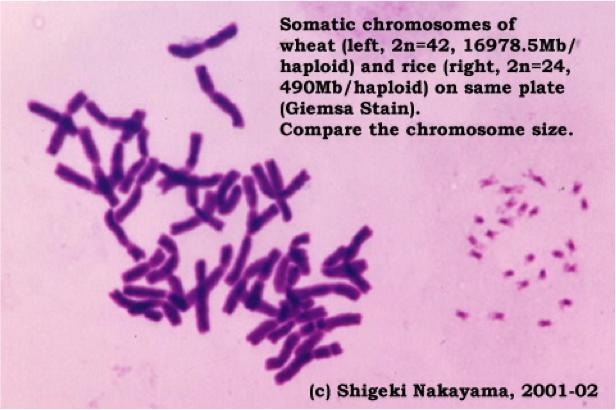
\includegraphics[width=0.7\textwidth]{images/wheat_rice_chromosomes}
  \end{center}  
\end{frame}

%
\begin{frame}
  \frametitle{Chromosome count/size
    \footnote{\tiny{Kamisugi \textit{et al}. (1993) \textit{Chromosome Res.} \textbf{1}(3): 189-196
}}
    \footnote{\tiny{\href{http://dx.doi.org/10.1038/nrg3375
}{Wang \textit{et al}. (2013) \textit{Nat. Rev. Genet.} doi:10.1038/nrg3375
}}}
  }
    \begin{itemize}
      \item \textcolor{hutton_green}{chromosome count and ploidy can vary widely} \\
        \begin{table}
		  \begin{tabular}{l | c | c }
		    Organism & Chromosomes & Ploidy  \\
			\hline \hline
			\textit{E. coli} & 1 & 1  \\ 
			Human (\textit{H. sapiens}) & 46 & 2 \\
			\hline
			Rice (\textit{O. sativa}) & 24 & 1  \\
			Adders-tongue & & \\ 
			(\textit{Ophioglossum reticulatum}) & 1260 & 84 \\
			\hline
			Domestic (not wild) wheat somatic & 42 & 6 \\
			Domestic (not wild) wheat gametic & 14 & 2 \\			
		  \end{tabular}
		\end{table}
	\end{itemize}
  \begin{center}
    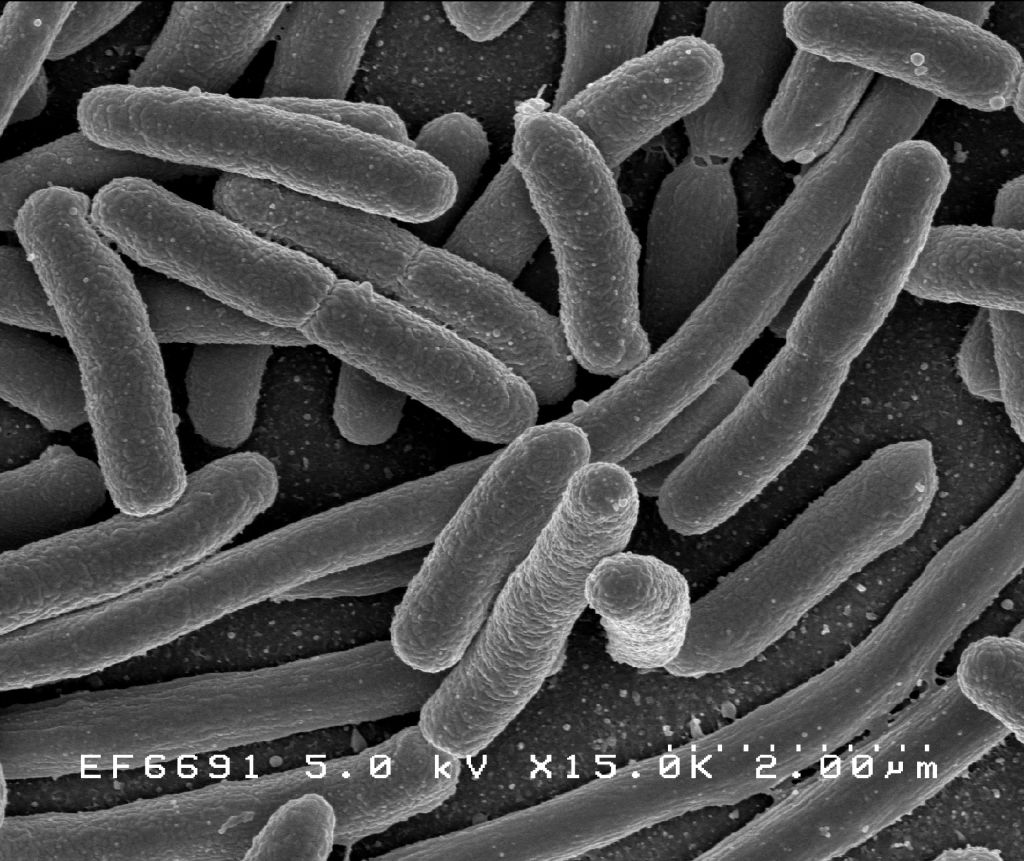
\includegraphics[height=0.15\textheight]{images/EscherichiaColi_NIAID}
    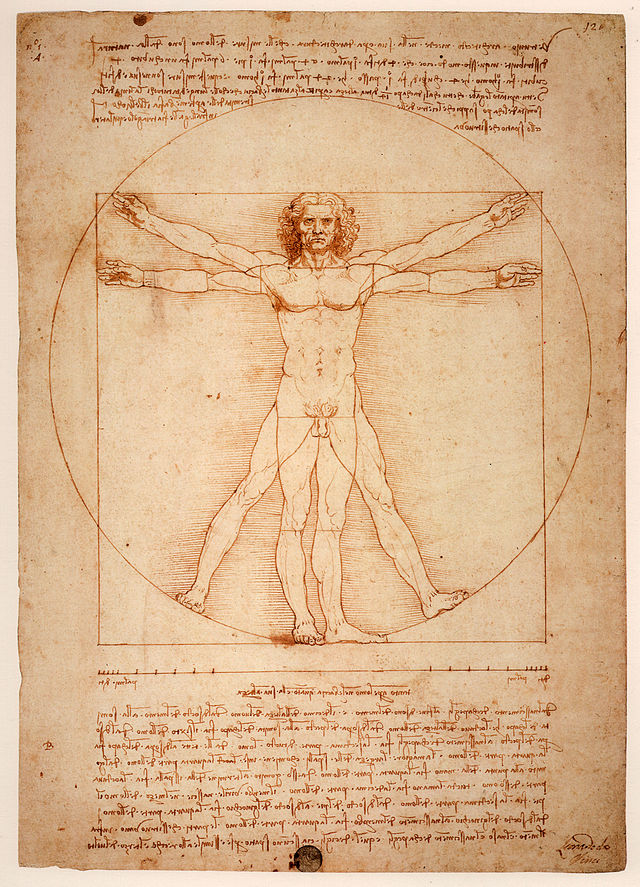
\includegraphics[height=0.15\textheight]{images/640px-Uomo_Vitruviano}
    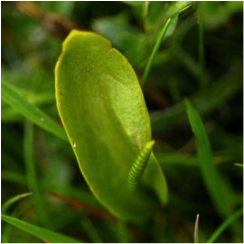
\includegraphics[height=0.15\textheight]{images/adders_tongue}
    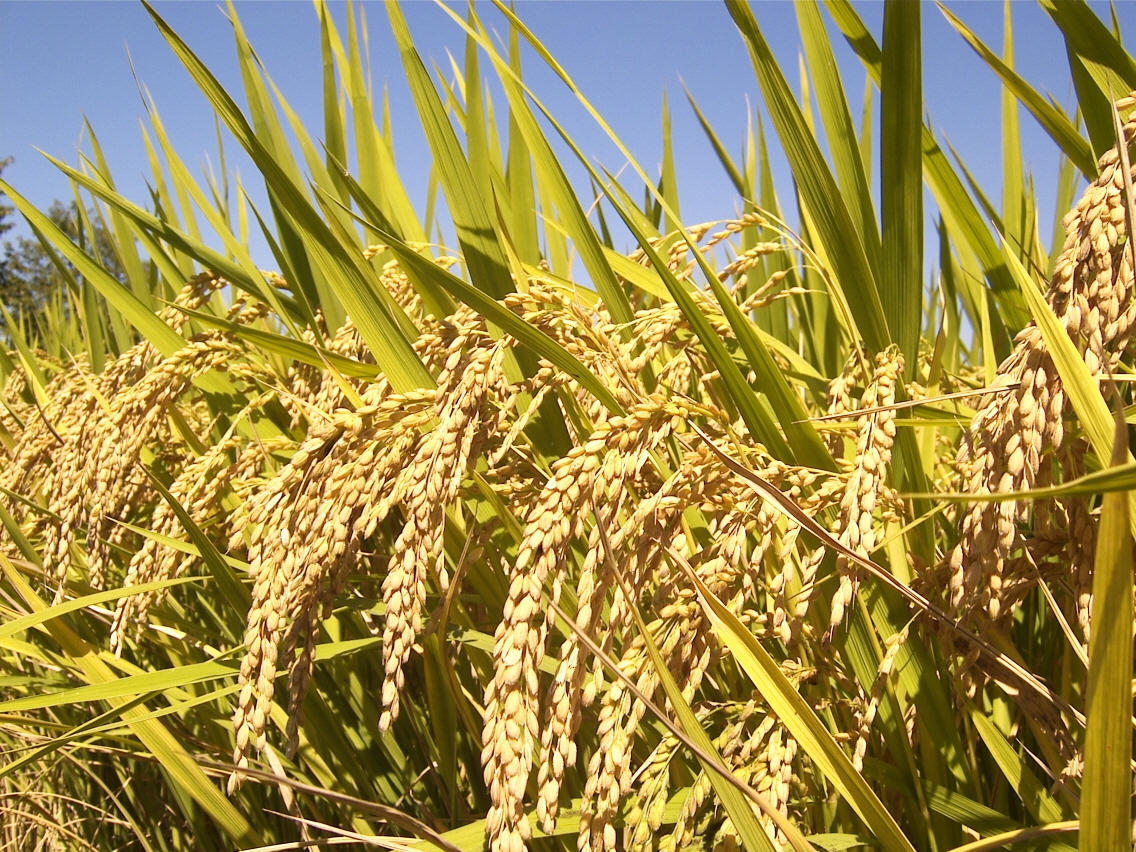
\includegraphics[height=0.15\textheight]{images/Rice_Plants_(IRRI)}
    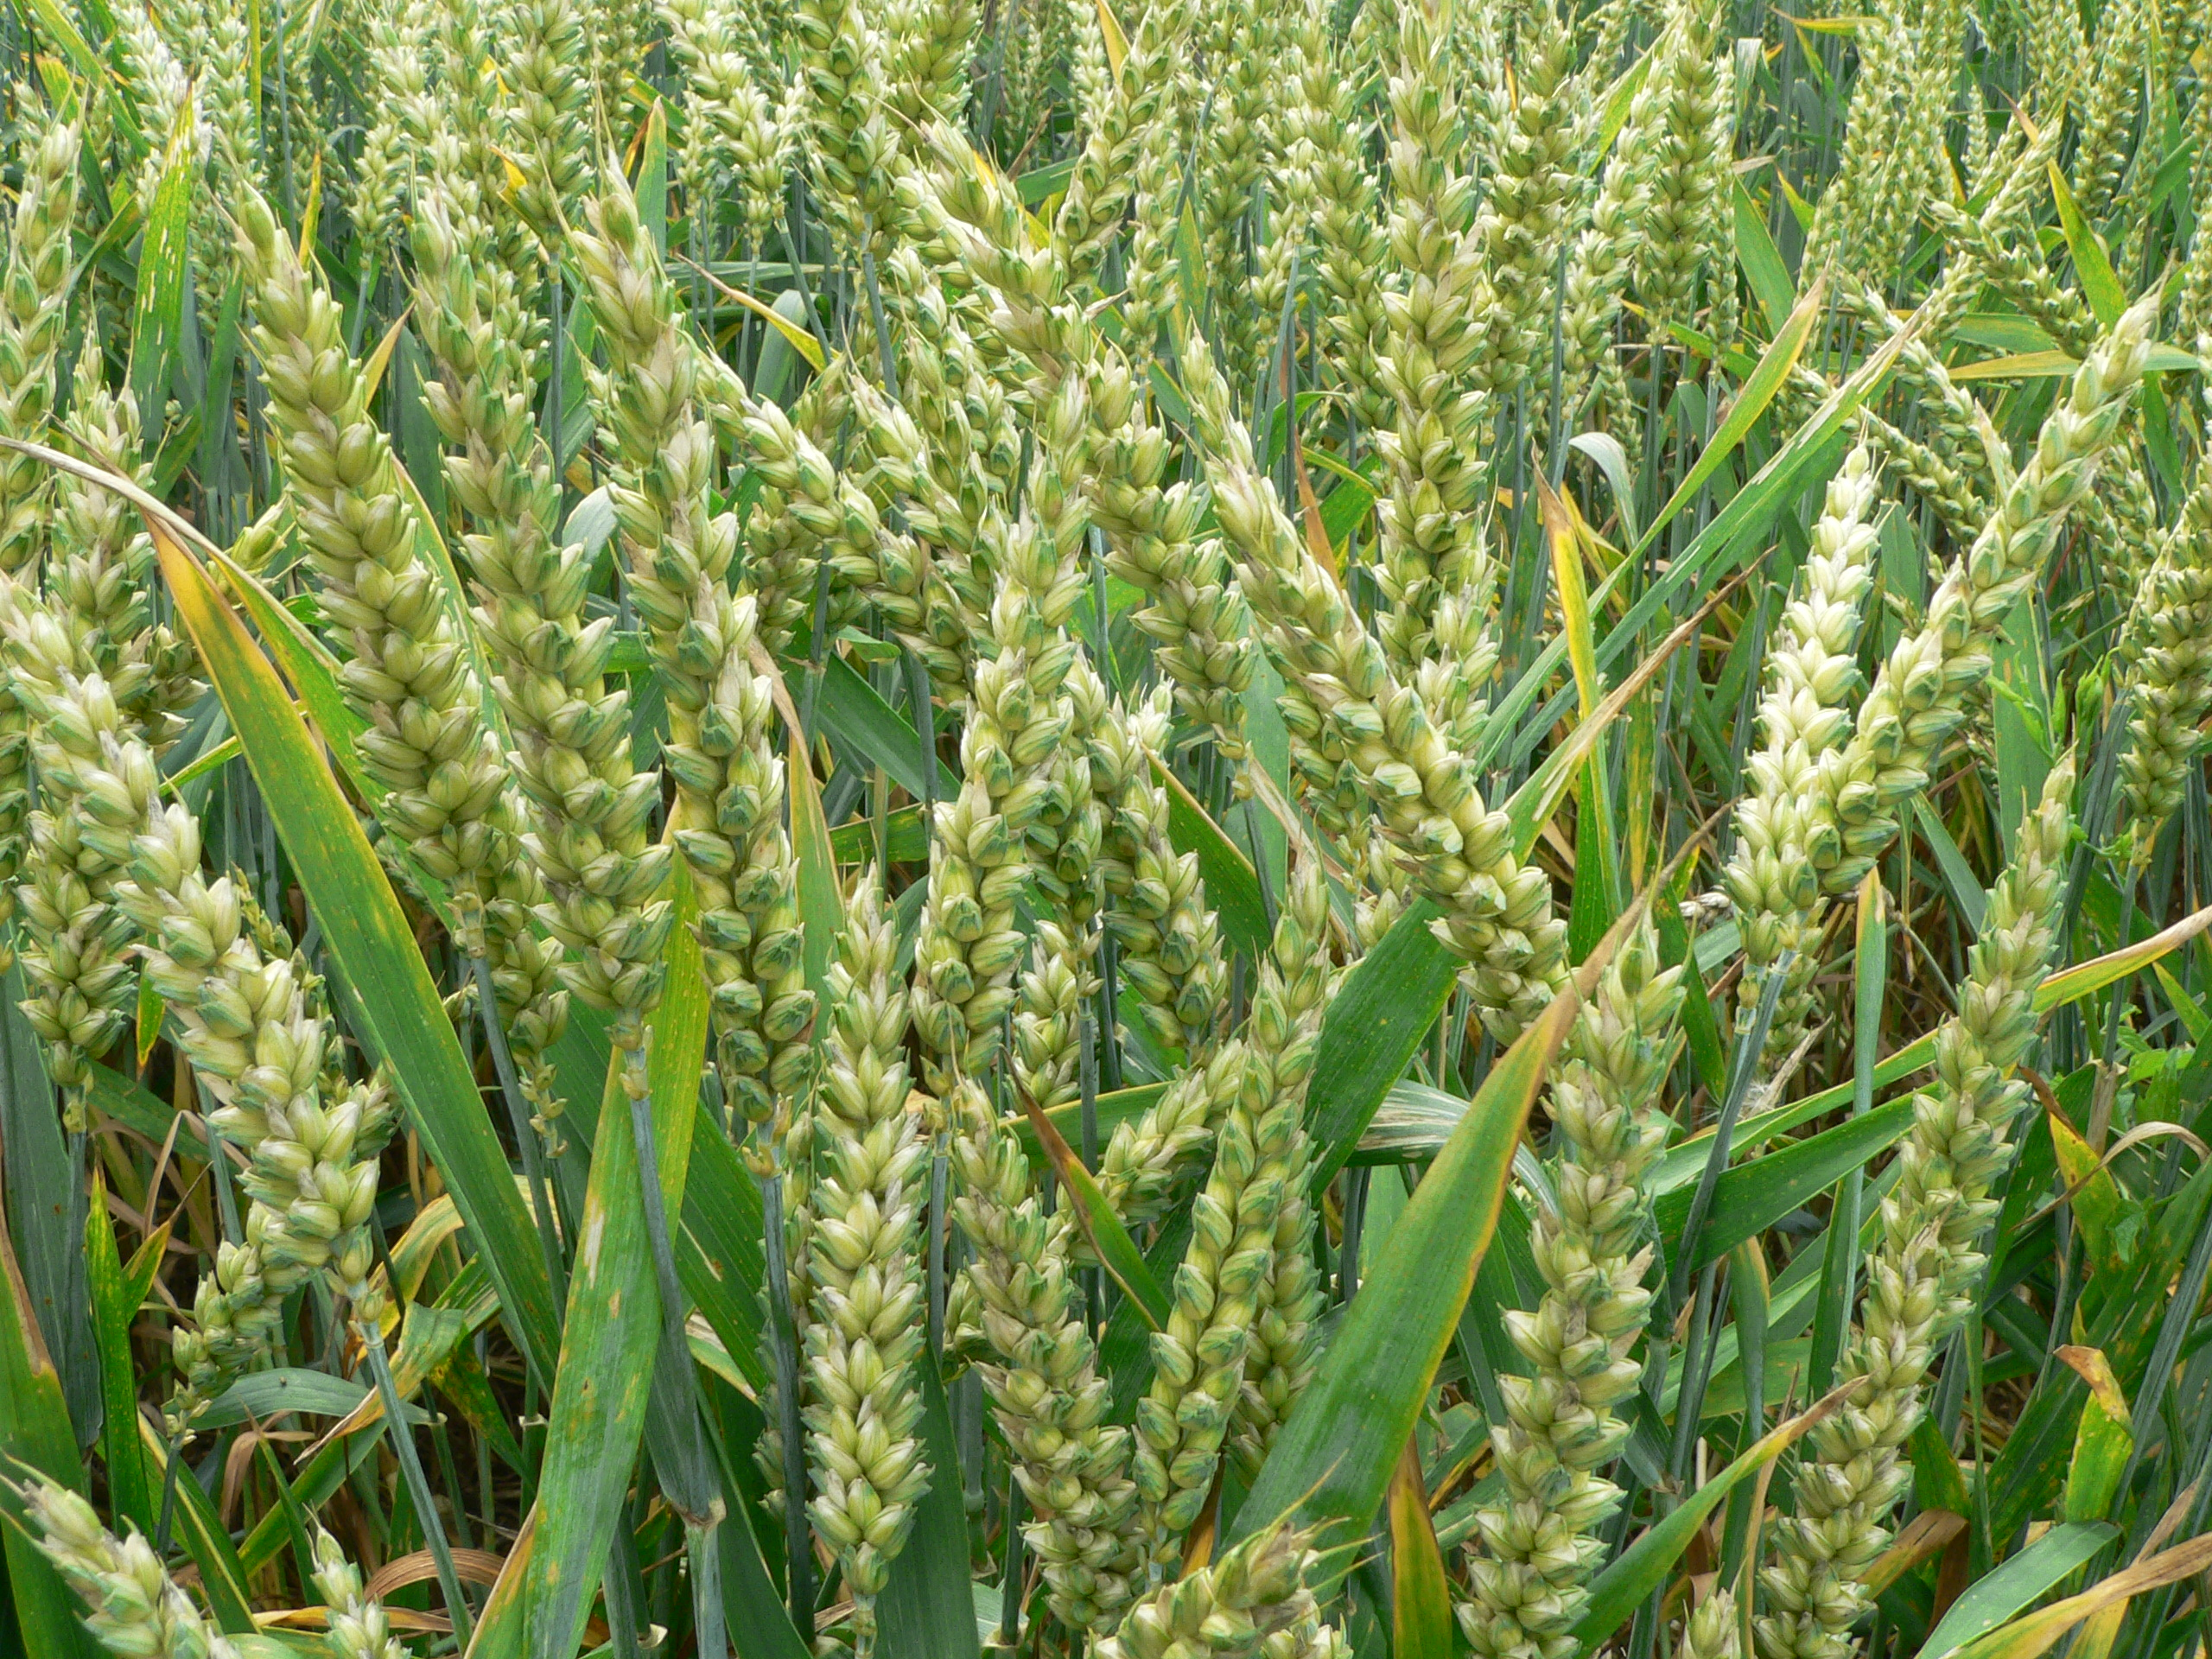
\includegraphics[height=0.15\textheight]{images/Wheat_P1210892}
  \end{center}  		
\end{frame}

%
\begin{frame}
  \frametitle{Physical study of chromosomes
  \footnote{\tiny{\href{http://dx.doi.org/10.1016/j.ymeth.2012.05.001
}{Belton \textit{et al}. (2012) \textit{Methods} doi:10.1016/j.ymeth.2012.05.001
}}}
  }
  \begin{itemize}
    \item \textcolor{hutton_green}{Genome size and chromosome count do \textbf{not} indicate organism ``complexity''}
    \item \textcolor{hutton_blue}{Modern physical study of chromosomes still produces surprises (e.g. Hi-C: chromatin interaction)}
  \end{itemize}
  \begin{center}
    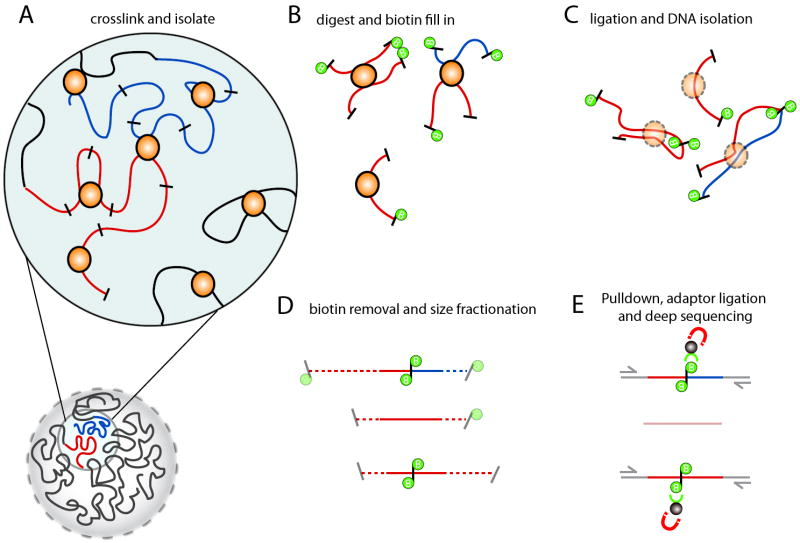
\includegraphics[width=0.7\textwidth]{images/nihms418977f1}
  \end{center}  
\end{frame}

%
\begin{frame}
  \frametitle{Nucleotide content
  \footnote{\tiny{Krane \textit{et al}. (1991) \textit{Nucl. Acids Res.} \textbf{19}(19): 5181-5185
}}
  }
  \begin{itemize}
    \item \textcolor{hutton_green}{Radiolabel monophosphates from genomic DNA}
    \item \textcolor{hutton_blue}{Separate by thin-layer chromatography}
    \item \textcolor{hutton_purple}{Compare label ratios using scanner}    
  \end{itemize}
  \begin{center}
    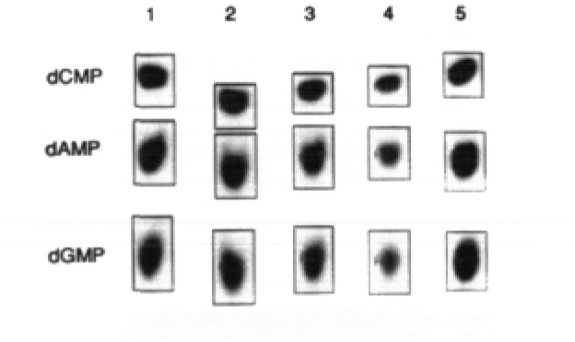
\includegraphics[height=0.4\textheight]{images/nucleotide_tlc}
    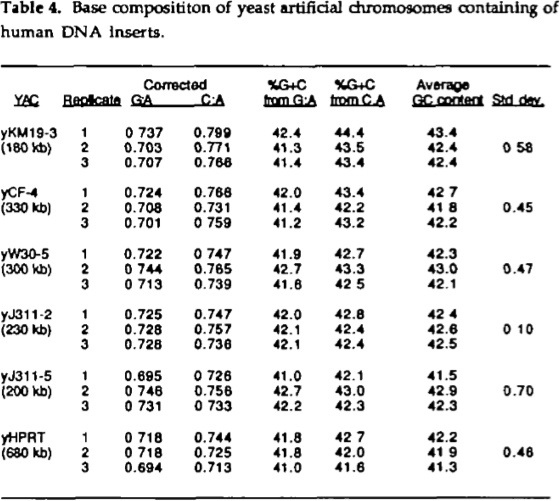
\includegraphics[height=0.4\textheight]{images/nucleotide_table}    
  \end{center}  
\end{frame}

%%
%\begin{frame}
%  \frametitle{Isochores
%  \footnote{\tiny{\href{http://dx.doi.org/10.1083/jcb.146.6.1211
%}{Sadoni \textit{et al}. (1999) \textit{J. Cell. Biol.} doi:10.1016/10.1083/jcb.146.6.1211
%}}}  
%  }
%    \begin{columns}[c] 
%      \column{.5\textwidth} 
%        \begin{itemize}
%         \item \textcolor{hutton_green}{ACGT composition varies within and between genomes}
%         \item \textcolor{RawSienna}{variation identified by staining}
%         \item \textcolor{hutton_blue}{\textit{isochore}: region with little internal GC variation}
%         \item \textcolor{hutton_purple}{In humans:}
%         \begin{itemize}
%           \item L1, L2: low GC ($\leq 41\%$)
%           \item H1, H2, H3: high GC ($\geq 41\%$)           
%         \end{itemize}
%        \end{itemize}
%      \column{.5\textwidth}
%        \begin{figure}
%        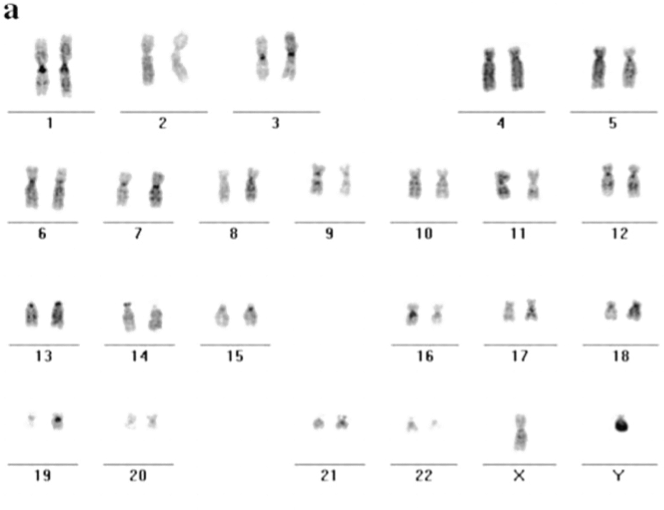
\includegraphics[width=\textwidth]{images/h3_isochores}
%        \caption{H3 isochore, human}
%        \end{figure}
%    \end{columns}  
%\end{frame}

% SUBSECTION
% Computational comparisons
\subsection{The impact of high throughput sequencing}
%% sequencing_impact.tex
%% Author: Leighton Pritchard
%% Copyright: James Hutton Institute
%% The impact high-throughput sequencing had

%
\begin{frame}
  \frametitle{This happened$\ldots$}
  \begin{itemize}
    \item Cheap, accurate, high-throughput sequencing
  \end{itemize}
  \begin{center}
    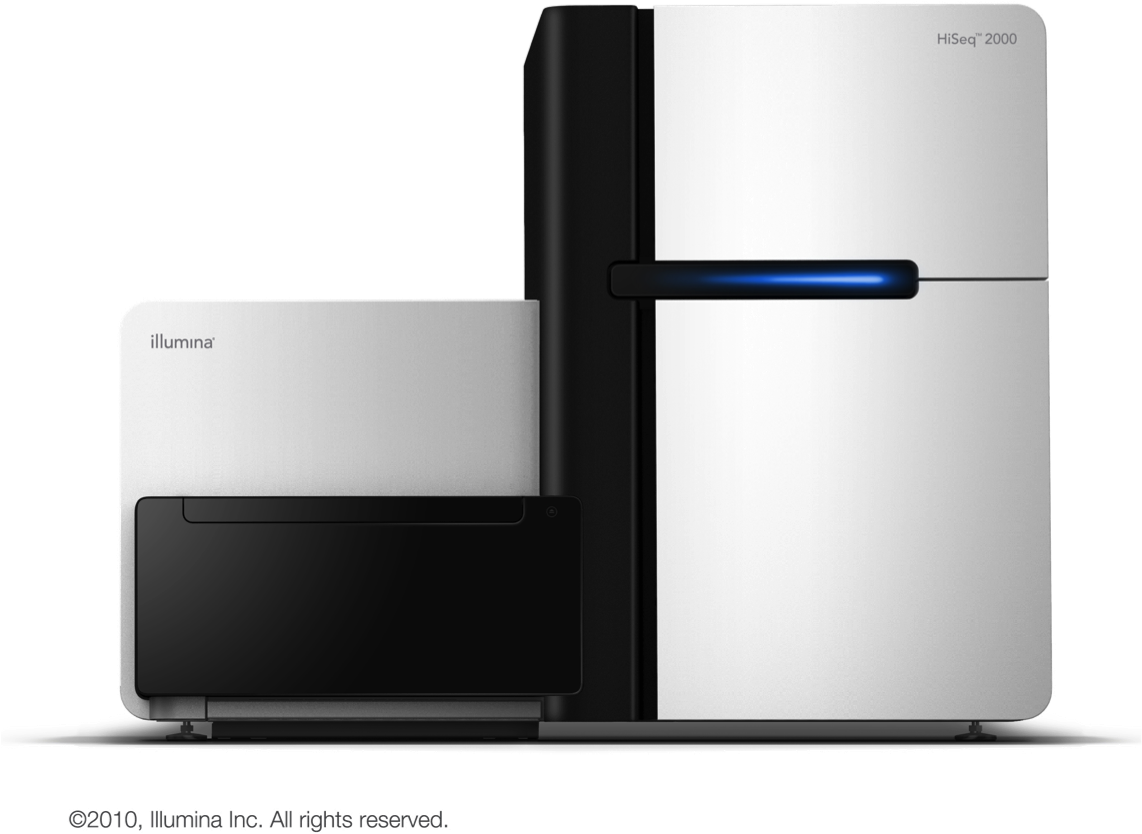
\includegraphics[width=0.7\textwidth]{images/illumina_hiseq}
  \end{center}  
\end{frame}

% Broad differences in chemistry and output
\begin{frame}
  \frametitle{Four different chemistries
\footnote{\tiny{Loman \textit{et al}. (2012) \textit{Nat. Rev. Micro.} \textbf{31}:294-296 \href{http://dx.doi.org/10.1038/nbt.2522}{doi:10.1038/nbt.2522
}}}
}
  Reads differ by technology, and can require different bioinformatic treatment$\ldots$
  \begin{itemize}
    \item \textcolor{hutton_green}{\textbf{Roche/454}: Pyrosequencing (long reads, but expensive, and high homopolymer errors) (700-800bp, 0.7Gbp, 23h)}
    \item \textcolor{hutton_blue}{\textbf{Illumina}: Reversible terminator (cost-effective, massive throughput, but short read lengths) (2x150bp, 1.5Gbp, 27h)}
    \item \textcolor{RawSienna}{\textbf{Ion Torrent}: Proton detection (short run times, good throughput, high homopolymers errors) (200bp, 1Gbp, 3h)}
    \item \textcolor{hutton_purple}{\textbf{PacBio}: Real-time sequencing (very long reads, high error rate, expensive) (3-15kbp, 3Gbp/day, 20min)}
  \end{itemize}
  $\ldots$ different error profiles, varying capability to assemble/determine variation
\end{frame}

% Sequencer relative costs
\begin{frame}
  \frametitle{Costs of sequencing\footnote{\tiny{Miyamoto \textit{et al}. (2014) \textit{BMC Genomics} \textbf{15}:699 \href{http://dx.doi.org/10.1186/1471-2164-15-699}{doi:10.1186/1471-2164-15-699}}}}
    \begin{center}
      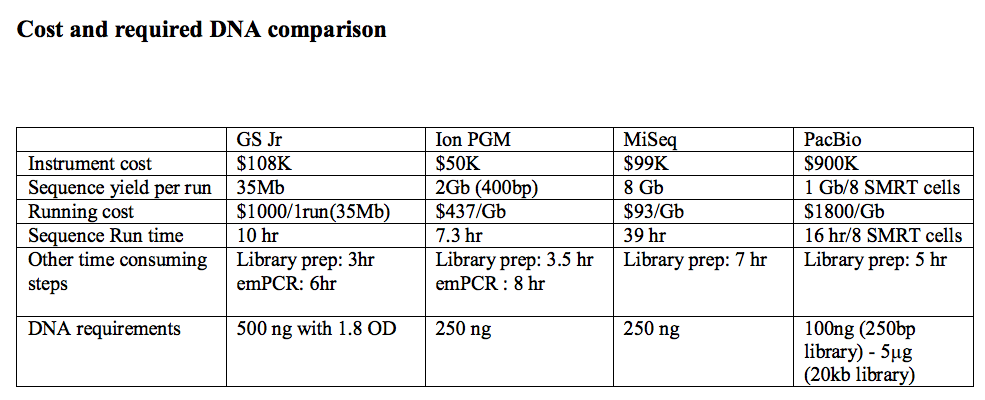
\includegraphics[width=1\textwidth]{images/miyamoto_costs}
    \end{center}      
\end{frame}

% How many genomes do we have, now?
\begin{frame}
  \frametitle{After that, the flood$\ldots$}
  High-throughput sequencing methods have completely changed the landscape of biology \\
  \textbf{(Nearly) complete, (mainly) accurate sequence data is now inexpensive} (and cheaper than analysis)
  \begin{itemize}
    \item \textcolor{hutton_green}{\href{http://www.genomesonline.org/cgi-bin/GOLD/index.cgi?page_requested=Complete+Genome+Projects&subset_requested=Complete+And+Published}{GOLD} (19/2/2014): 3,011 ``finished'' ; 9,891 ``permanent draft'' genomes}
    \item \textcolor{hutton_blue}{\href{http://www.genomesonline.org/cgi-bin/GOLD/index.cgi?page_requested=Complete+Genome+Projects&subset_requested=Complete+And+Published}{GOLD} (18/11/2014): 6,649 ``finished'' ; 23,552 ``permanent draft'' genomes}
    \item \textcolor{RawSienna}{\href{http://www.ncbi.nlm.nih.gov/Traces/wgs/}{NCBI WGS} (19/2/2014): 17,023 microbial genomes}
    \item \textcolor{hutton_purple}{\href{http://www.ncbi.nlm.nih.gov/Traces/wgs/}{NCBI WGS} (18/11/2014): 26,026 microbial genomes}
  \end{itemize}
\end{frame}

% And how many are we going to have?
\begin{frame}
  \frametitle{Predicting the future is hard$\ldots$}
    Su \textit{et al}. attempted to answer this\footnote{\tiny{\href{http://sulab.org/2013/06/sequenced-genomes-per-year/}{http://sulab.org/2013/06/sequenced-genomes-per-year/}}}:
    \begin{center}
      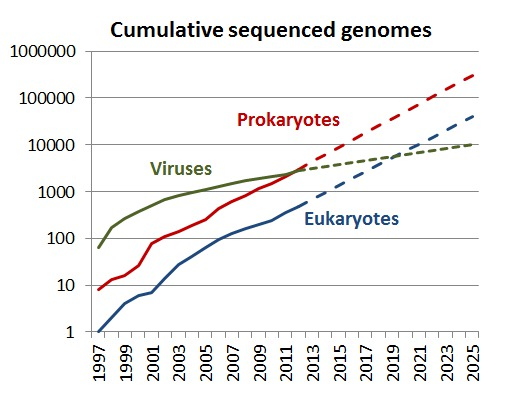
\includegraphics[width=0.5\textwidth]{images/cumulative_sequenced_genomes1}
      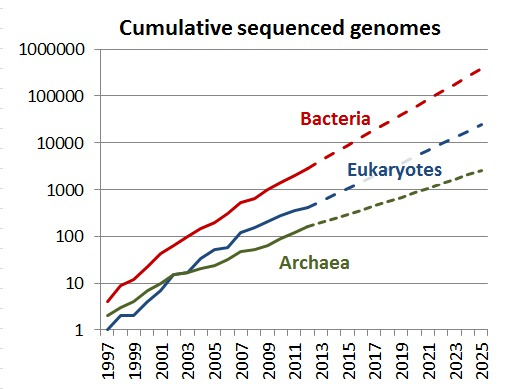
\includegraphics[width=0.5\textwidth]{images/cumulative_sequenced_genomes2}
    \end{center}     
%    How will we keep this much genomic data well-organised?
\end{frame}

% Nanopore
\begin{frame}
  \frametitle{What's coming next?}
  Oxford Nanopore. A sequencer the size of your hand.
    \begin{center}
      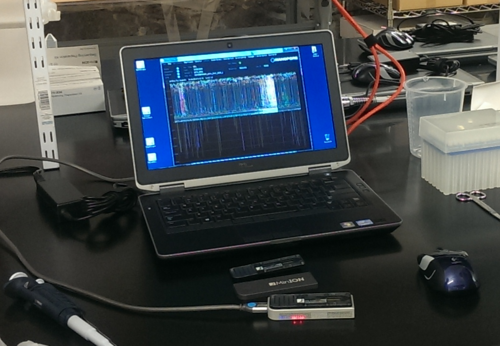
\includegraphics[width=0.48\textwidth]{images/minion_run}\thinspace
      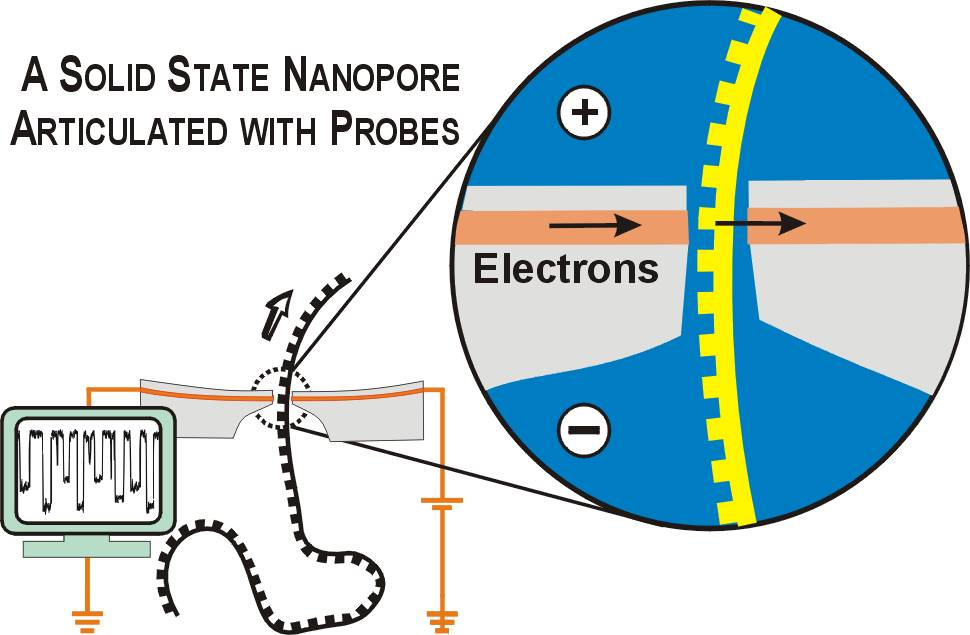
\includegraphics[width=0.48\textwidth]{images/nanopore_schematic}
    \end{center} 
    \begin{itemize}
      \item Microfluidics, single-molecule sequencing; 11-70kbp reads
      \item Reports current across pore (tiny electron microscope) as molecule moves through
      \item \$10/Mbp, 110Mbp per flowcell\footnote{\tiny{Yaniv Erlich (2013) \href{http://erlichya.tumblr.com/post/66376172948/hands-on-experience-with-oxford-nanopore-minion}{Future Continuous blog}}}
    \end{itemize}          
\end{frame}
% SUBSECTION
% Computational comparisons
\subsection{In silico bulk genome comparisons}
%% bulk_genome_comparisons_comp.tex
%% Author: Leighton Pritchard
%% Copyright: James Hutton Institute
%% Bulk genome comparisons - computational

%
\begin{frame}
  \frametitle{Bulk genome comparisons}
  \Large{
    \textcolor{olive}{
      \textbf{
      You don't have to sequence genomes to compare them \\
      (but it helps) \\
      PART 2: \textit{in silico}
      }
    }
  }
\end{frame}

%
\begin{frame}
  \frametitle{Bulk genome comparisons}
  \Large{
    \textcolor{hutton_blue}{
      \textbf{
      EXERCISE 1: \\
      \url{ex01_gc_content.ipynb}
      }
    }
  }
\end{frame}

%
\begin{frame}
  \frametitle{Nucleotide frequency/genome size}
  Very easy to calculate from complete or draft genome sequence \\
  \begin{center}
    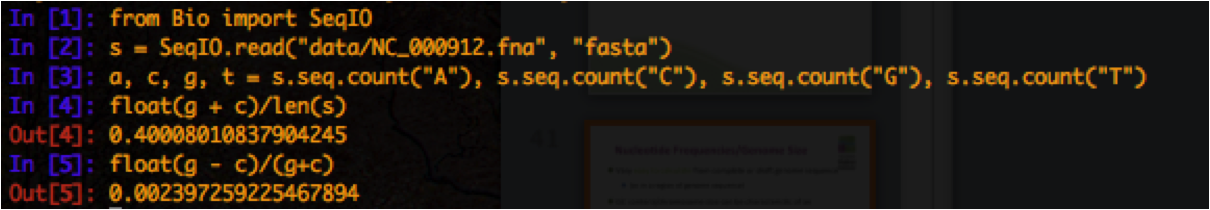
\includegraphics[width=\textwidth]{images/python_gc} \\
  \end{center}  
  GC content, chromosome size can be characteristic of an organism.
\end{frame}

%
\begin{frame}
  \frametitle{Blobology
  \footnote{\tiny{\href{http://dx.doi.org/10.1007/s13199-012-0154-6
}{Kumar \& Blaxter (2011) \textit{Symbiosis} doi:10.1007/s13199-012-0154-6
}}}
  \footnote{\tiny{\href{http://nematodes.org/bioinformatics/blobology/
}{http://nematodes.org/bioinformatics/blobology/
}}}  
  }
  Sequence data can be contaminated by other organisms
  \begin{itemize}
    \item \textcolor{hutton_green}{Host and symbiont DNA have different \%GC}
    \item \textcolor{hutton_green}{Host and symbiont DNA differ in coverage}
  \end{itemize}
  \begin{columns}[T] 
    \column{.6\textwidth} 
      \begin{itemize}
        \item \textcolor{RawSienna}{Assemble genome}
        \item \textcolor{hutton_blue}{Map reads}
        \item \textcolor{hutton_purple}{Plot coverage against \%GC}
      \end{itemize}
    \column{.4\textwidth}
      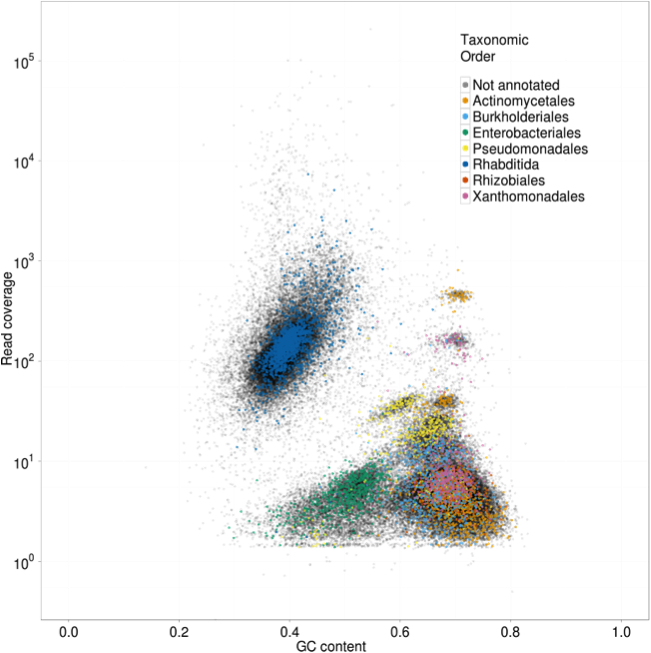
\includegraphics[width=\textwidth]{images/blobology}
  \end{columns}    
\end{frame}

%
\begin{frame}
  \frametitle{Nucleotide $k$-mers}
  Sequence data is necessary to determine $k$-mers/frequencies
  \begin{itemize}
    \item \textcolor{hutton_green}{Nucleotides, $k=1$, 4x1-mers} \\
      \url{A, C, G, T}
    \item \textcolor{hutton_blue}{Dinucleotides, $k=2$, 16x2-mers} \\
      \url{AA, AC, AG, AT, CA, CC, CG, CT, GA, GC, GG, GT, TA, TC, TG, TT}
    \item \textcolor{RawSienna}{Triucleotides, $k=1$, 64x3-mers}
    \item \textcolor{hutton_purple}{$k$-nucleotides, $4^k$x$k$-mers}
  \end{itemize}  
\end{frame}

%
\begin{frame}
  \frametitle{Finding $k$-mers}
  \Large{
    \textcolor{hutton_blue}{
      \textbf{
      ACTIVITY: \\
      \small{
        \href{https://widdowquinn.shinyapps.io/nucleotide_frequencies/}{https://widdowquinn.shinyapps.io/nucleotide\_frequencies/}
        }
      }
    }
  }
\end{frame}

%
\begin{frame}
  \frametitle{$k$-mer spectra
  \footnote{\tiny{\href{http://dx.doi.org/10.1186/gb-2009-10-10-r108
}{Chor \textit{et al.} (2009) \textit{Genome Biol.} doi:10.1186/gb-2009-10-10-r108
}}}
  }
  \textcolor{RawSienna}{$k$-mer spectrum: frequency distribution of observed $k$-mer counts.} \\
  Most species have a unimodal $k$-mer spectrum
  \begin{center}
    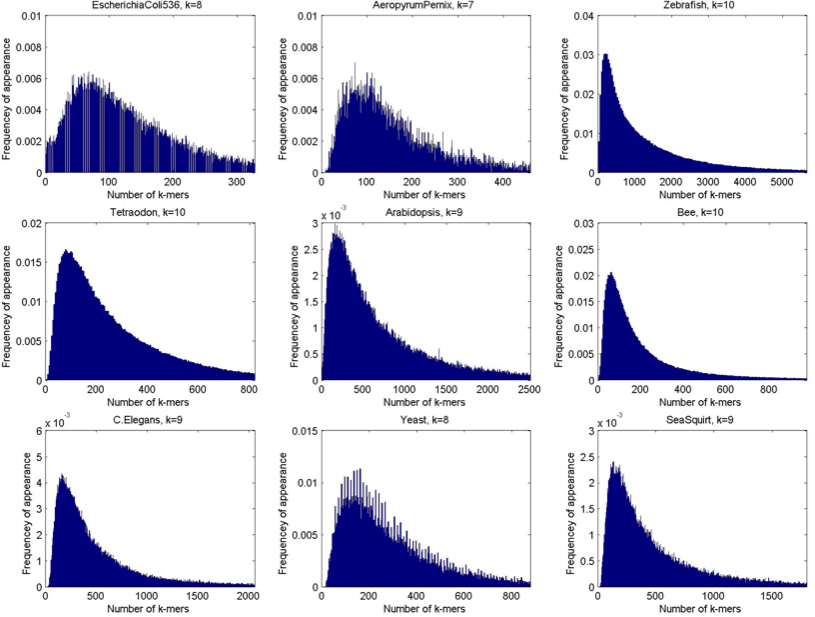
\includegraphics[height=0.6\textheight]{images/kmer_spectra} \\
  \end{center}  
\end{frame}

%
\begin{frame}
  \frametitle{Bulk genome comparisons}
  \Large{
    \textcolor{hutton_blue}{
      \textbf{
      EXERCISE 2: \\
      \url{ex02_kmer_spectra.ipynb}
      }
    }
  }
\end{frame}


%%%
% LICENCE FOR REUSE
%% licence.tex
%% Author: Leighton Pritchard
%% Copyright: James Hutton Institute
%% These slides describe the licence for reuse of these slides and
%% materials

%
\begin{frame}
  \frametitle{Licence: CC-BY-SA}
  By: Leighton Pritchard \\[0.5cm]
  This presentation is licensed under the Creative Commons Attribution ShareAlike license \\
  \href{https://creativecommons.org/licenses/by-sa/4.0/}{https://creativecommons.org/licenses/by-sa/4.0/}
\end{frame}

% etc
\end{document}